\newpage
\section{3 Dimensional Analysis}
\noindent This section is an extended analysis of the 2 dimensional analyses which intended to explore and analyse the 3 dimensional flow feature. It was surmised that the 3 dimensional flow offer a complex flow behaviour that may significantly affect overall performance of an undertray. This part of the paper will be divided into 3D open-flow and undertray prototype with bluff body analyses.


\subsection{3D Open-Flow}
\subsubsection{Overview}
This analysis is the extension of 3 dimensional analysis of 2D open-flow. This analysis is purposed to investigate further flow features of an undertray which may affect its performance based on similar variable as previous.

\subsubsection{Geometry and Mesh generation}
An identical 2D sketch from geometry 3 - 2D open flow was used, which then extruded to 0.5 meters thickness with skirt on both side of the rear diffuser. Fences were also added on the next analyses to investigate the effect of vortex generator on downforce generation. 

\begin{figure}[!h]
    \centering
    \noindent\makebox[\textwidth]{
    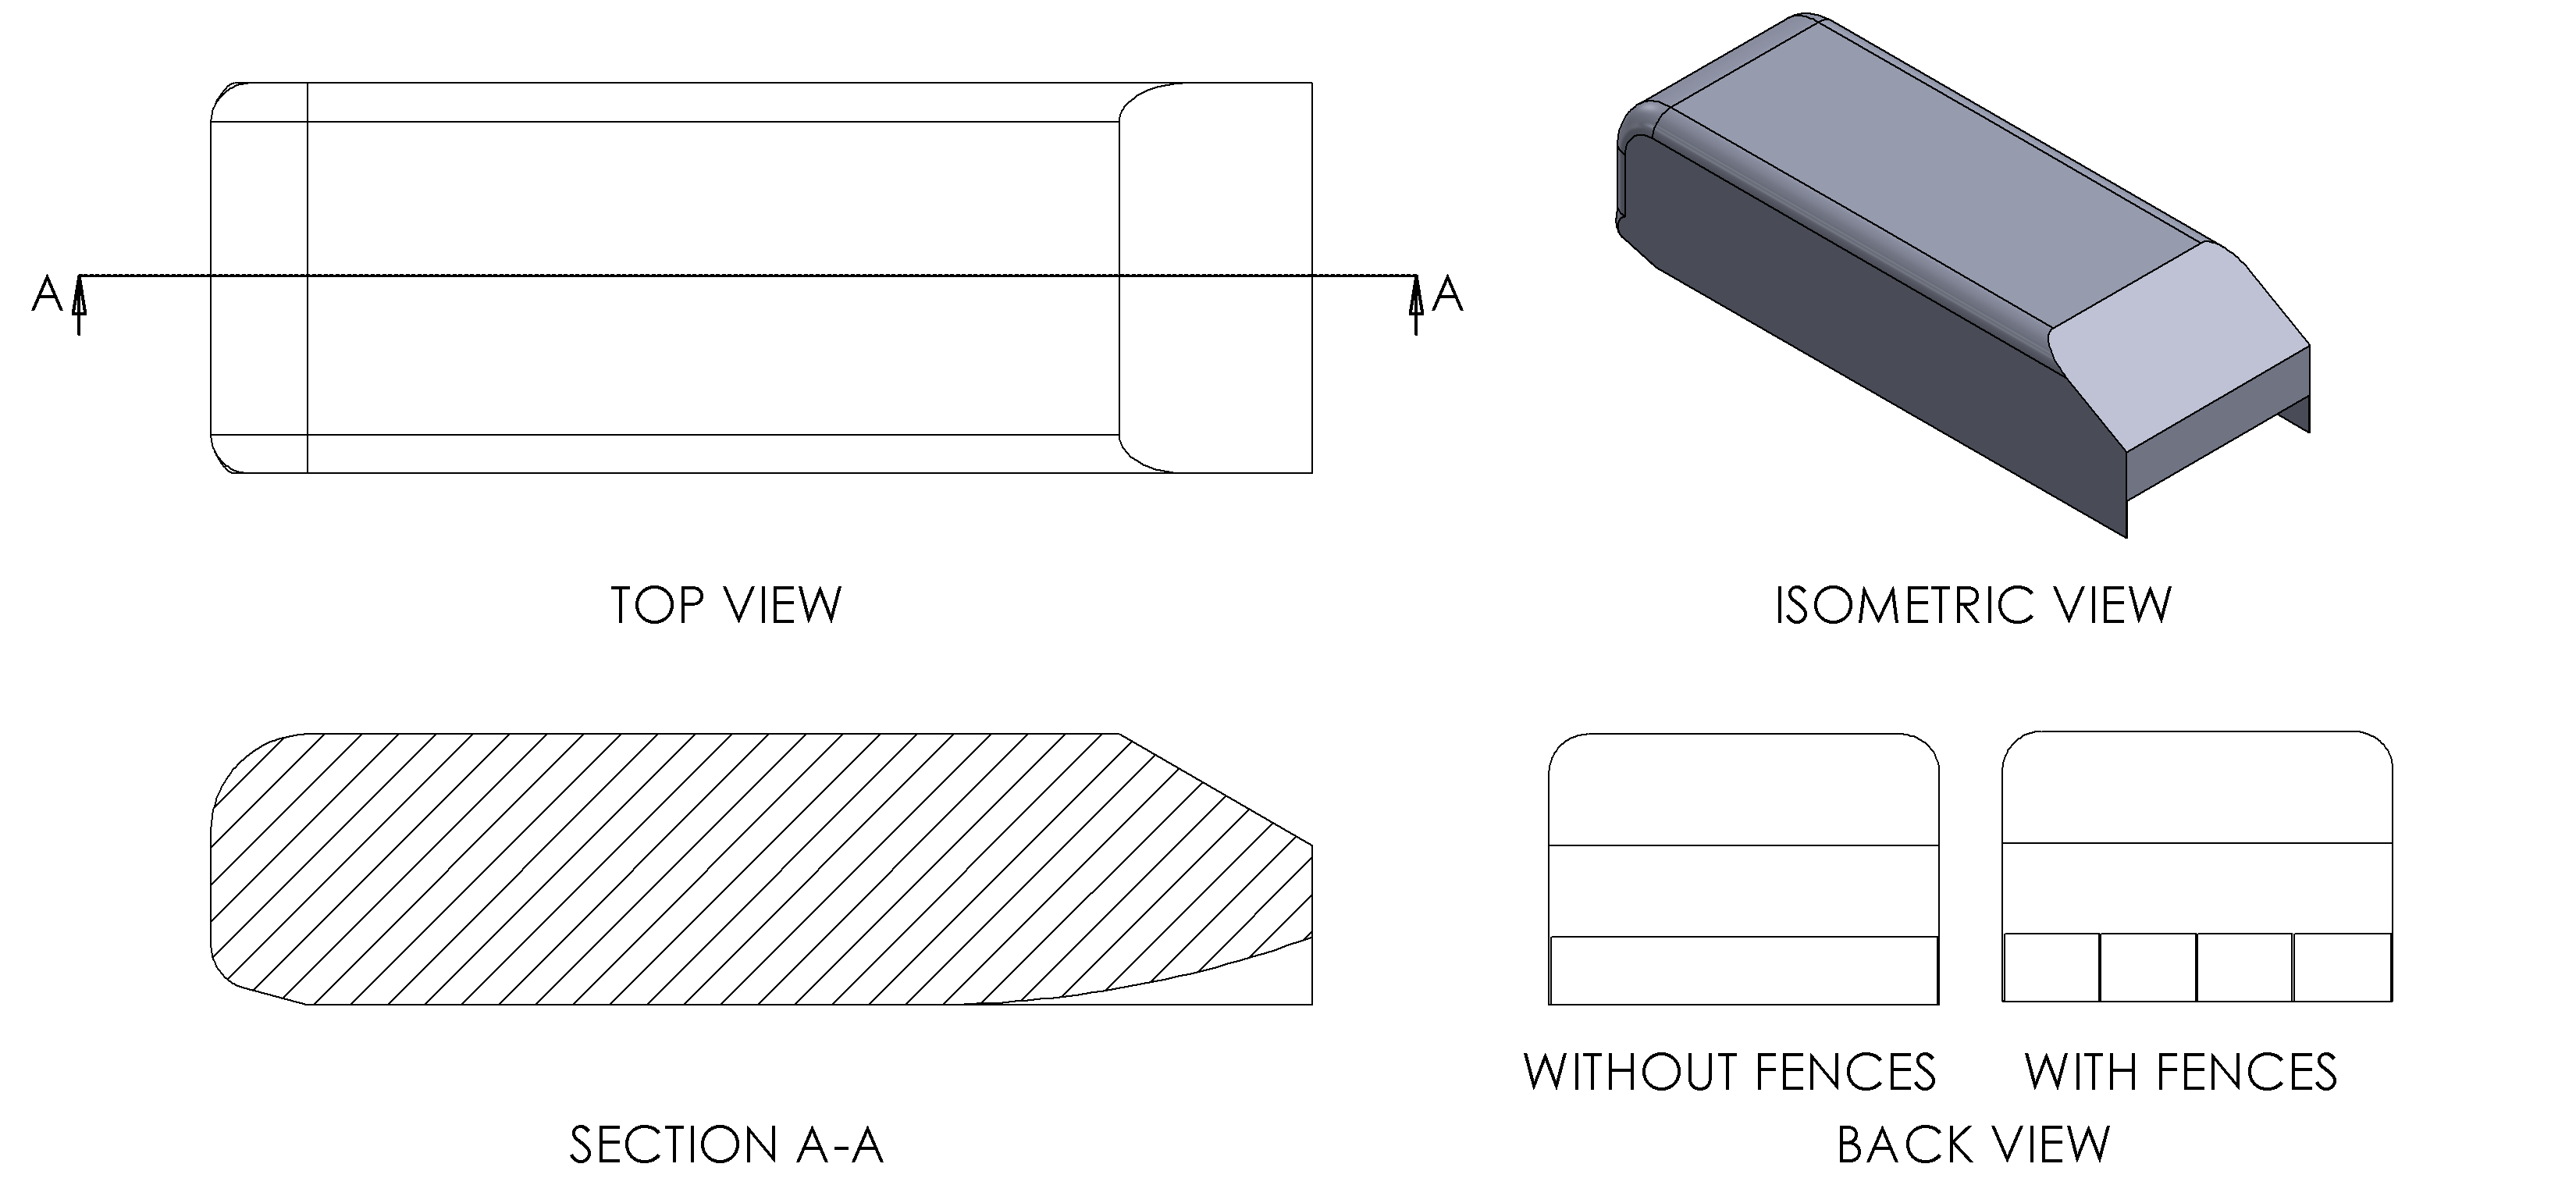
\includegraphics[width=1\textwidth]{Figures/3D_OF/3D_OF_D.PNG}}
    \caption{Geometry generated for 3D open-flow analyis.}
    \label{fig:3D_OF_GEOM}
\end{figure}

\subsection{3D Undertray}
